\titledquestion{Lexical analysis}
\droptotalpoints

Let $G_2$ be a formal grammar with nonterminal symbols $S$ and $D$,
terminal symbols '$\mathbf{b}$', '$\mathbf{0}$' and '$\mathbf{1}$', 
start symbol $S$, and the following production rules:
\begin{eqnarray*}
S & \rightarrow & \mathbf{b\ } D\\
D & \rightarrow & \mathbf{0\ } D\\
D & \rightarrow & \mathbf{1\ } D\\
D & \rightarrow & \mathbf{0}\\
D & \rightarrow & \mathbf{1}
\end{eqnarray*}

\begin{parts}

\part[1]
Is $G_2$ regular? Why (not)?

\begin{solution}
Yes.
All rules have only a single nonterminal symbol on their left-hand side and
either a single terminal symbol or a terminal symbol followed by a nonterminal
symbol on their right-hand side.
\end{solution}

\part[2]
Describe the language defined by $G_2$ in English.

\begin{solution}
The language consists of all words starting with \textbf{b}, followed by one or
more digits \textbf{0} or \textbf{1}, i.e. binary numbers marked with a leading
\textbf{b}.
\end{solution}

\part[4]
Turn $G_2$ \emph{systematically} into a finite automaton.

\begin{solution}
\vspace{-1em}
\begin{center}
  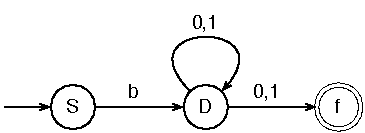
\includegraphics[scale=.85]{questions/lexical/binaries-nfa}
\end{center}
\end{solution}

\part[3]
Use $G_2$ to generate a word with at least five letters. 
Show each derivation step.
Use the automaton to recognise this word. 
Enumerate the states passed during the recognition.

\begin{solution}
\vspace{-1em}
\begin{displaymath}
S \Rightarrow 
\mathbf{b\ } D \Rightarrow 
\mathbf{b\ } \mathbf{1\ } D \Rightarrow 
\mathbf{b\ } \mathbf{1\ } \mathbf{0\ } D \Rightarrow 
\mathbf{b\ } \mathbf{1\ } \mathbf{0\ } \mathbf{1\ } D \Rightarrow 
\mathbf{b\ } \mathbf{1\ } \mathbf{0\ } \mathbf{1\ } \mathbf{0}
\end{displaymath}
\begin{displaymath}
S \stackrel{\mathbf{b}}{\rightarrow} 
D \stackrel{\mathbf{1}}{\rightarrow} 
D \stackrel{\mathbf{0}}{\rightarrow} 
D \stackrel{\mathbf{1}}{\rightarrow} 
D \stackrel{\mathbf{0}}{\rightarrow} 
f
\end{displaymath}

\end{solution}

\end{parts}
